%\documentclass[aspectratio=43]{beamer}
\documentclass[t]{beamer}
\usetheme{ffmodern}  %% Themenwahl

\usepackage[ngerman]{babel}
\usepackage[T1]{fontenc}    % richtige Silbentrennung
\usepackage[utf8]{inputenc} % Umlaute etc.!
\usepackage{eurosym}
\usepackage{tikz}
\usepackage{pgffor}
\usepackage{textcomp}
\usepackage{textpos}
\usepackage{tikz}
\usepackage{mathtools}
\usepackage{grid-system}
\usetikzlibrary{arrows,decorations.pathmorphing,backgrounds,fit,positioning,shapes.symbols,chains}

%-----------------
\title{Freifunk}
\author{Das freie WLAN-Netz} % TODO: anderer Untertitel? Bürgernetz?
\date{03. Mai 2017}
\license{CC-BY-3.0}

\begin{document}
  \maketitle

  %-----------------
  \begin{frame}{Was ist Freifunk?}
    \begin{columns}
      \begin{column}{0.75\textwidth}
        \hspace{0.75em}\Large{Initiative für freie (Funk-)Netze}
        \vspace{1em}
        \begin{itemize}
          \item \textbf{Nicht kommerziell}
          \item Mitmachnetz: \textbf{Netz in Nutzerhand}
          \item Gleichbehandlung aller Daten (\textbf{Netzneutralität})
          \item Infrastruktur \textbf{dezentral} organisiert
        \end{itemize}
      \end{column}
      \begin{column}{0.25\textwidth}
        \begin{center}
          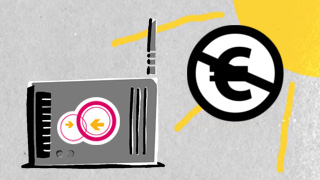
\includegraphics[width=\textwidth]{images/freifunk_insel_nc}\newline
          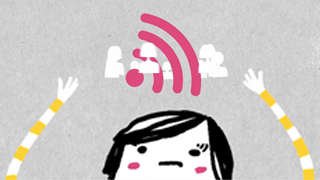
\includegraphics[width=\textwidth]{images/up}\newline
          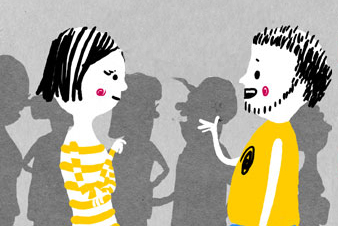
\includegraphics[width=\textwidth]{images/talk}
        \end{center}
      \end{column}
    \end{columns}
  \end{frame}

  %-----------------
  \begin{frame}{Was ist Freifunk?}
    \begin{center}
      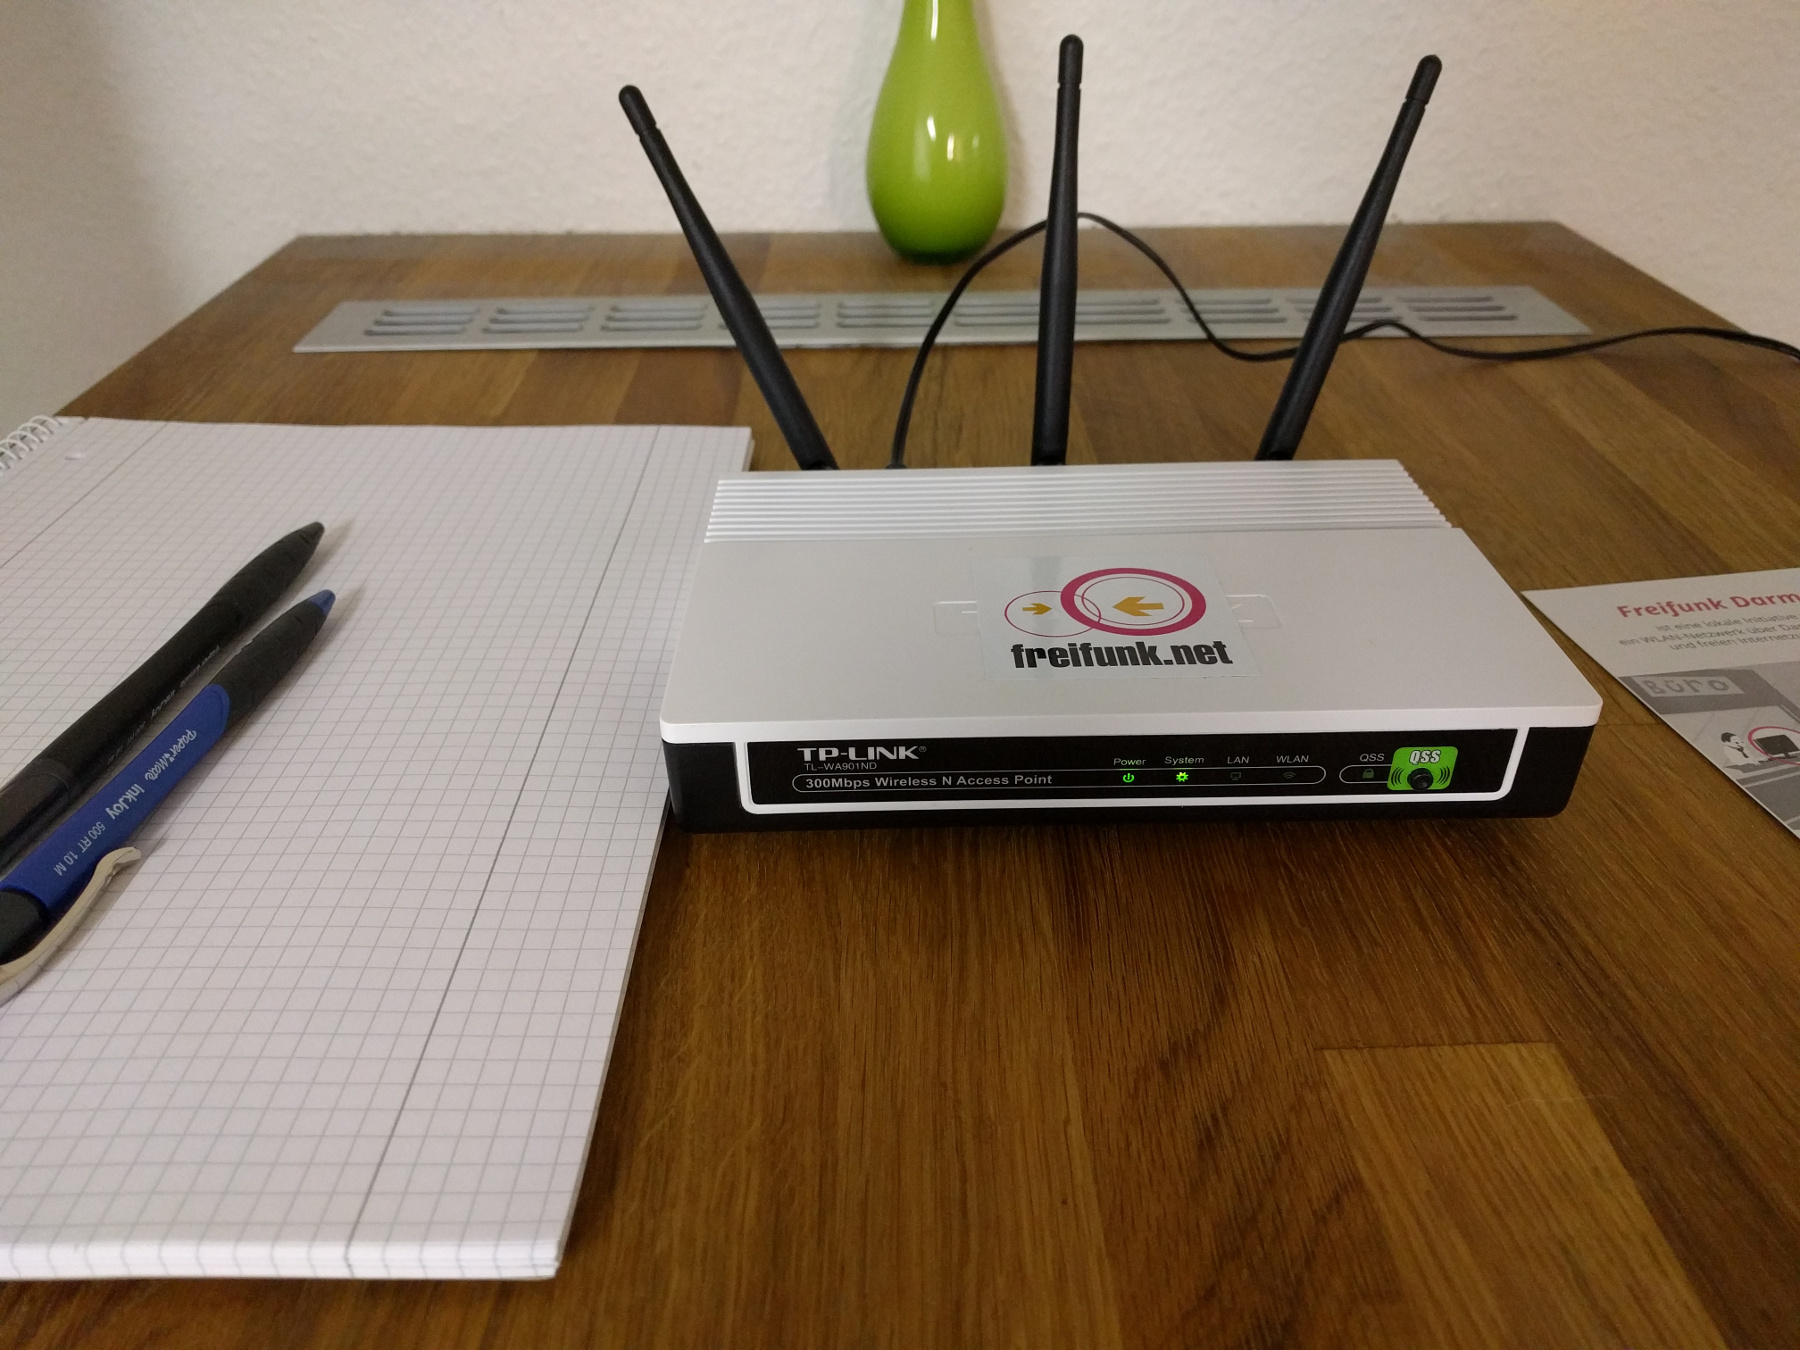
\includegraphics[width=7cm]{images/homerouter}
    \end{center}
  \end{frame}

  %-----------------
  \begin{frame}{Was ist Freifunk?}
    \begin{center}
      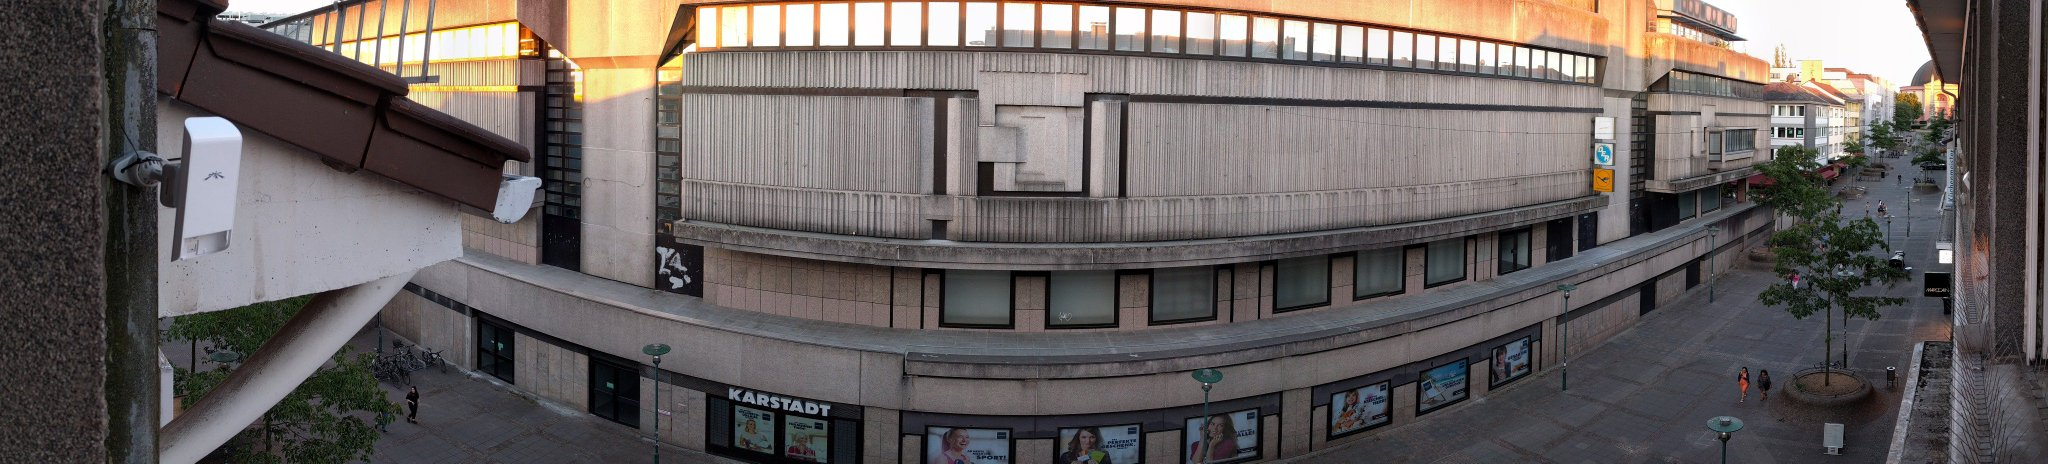
\includegraphics[width=10cm]{images/irl/wilhelminenstr1}
    \end{center}
  \end{frame}


  %-----------------
  \begin{frame}{Was ist Freifunk?}
    \begin{center}
      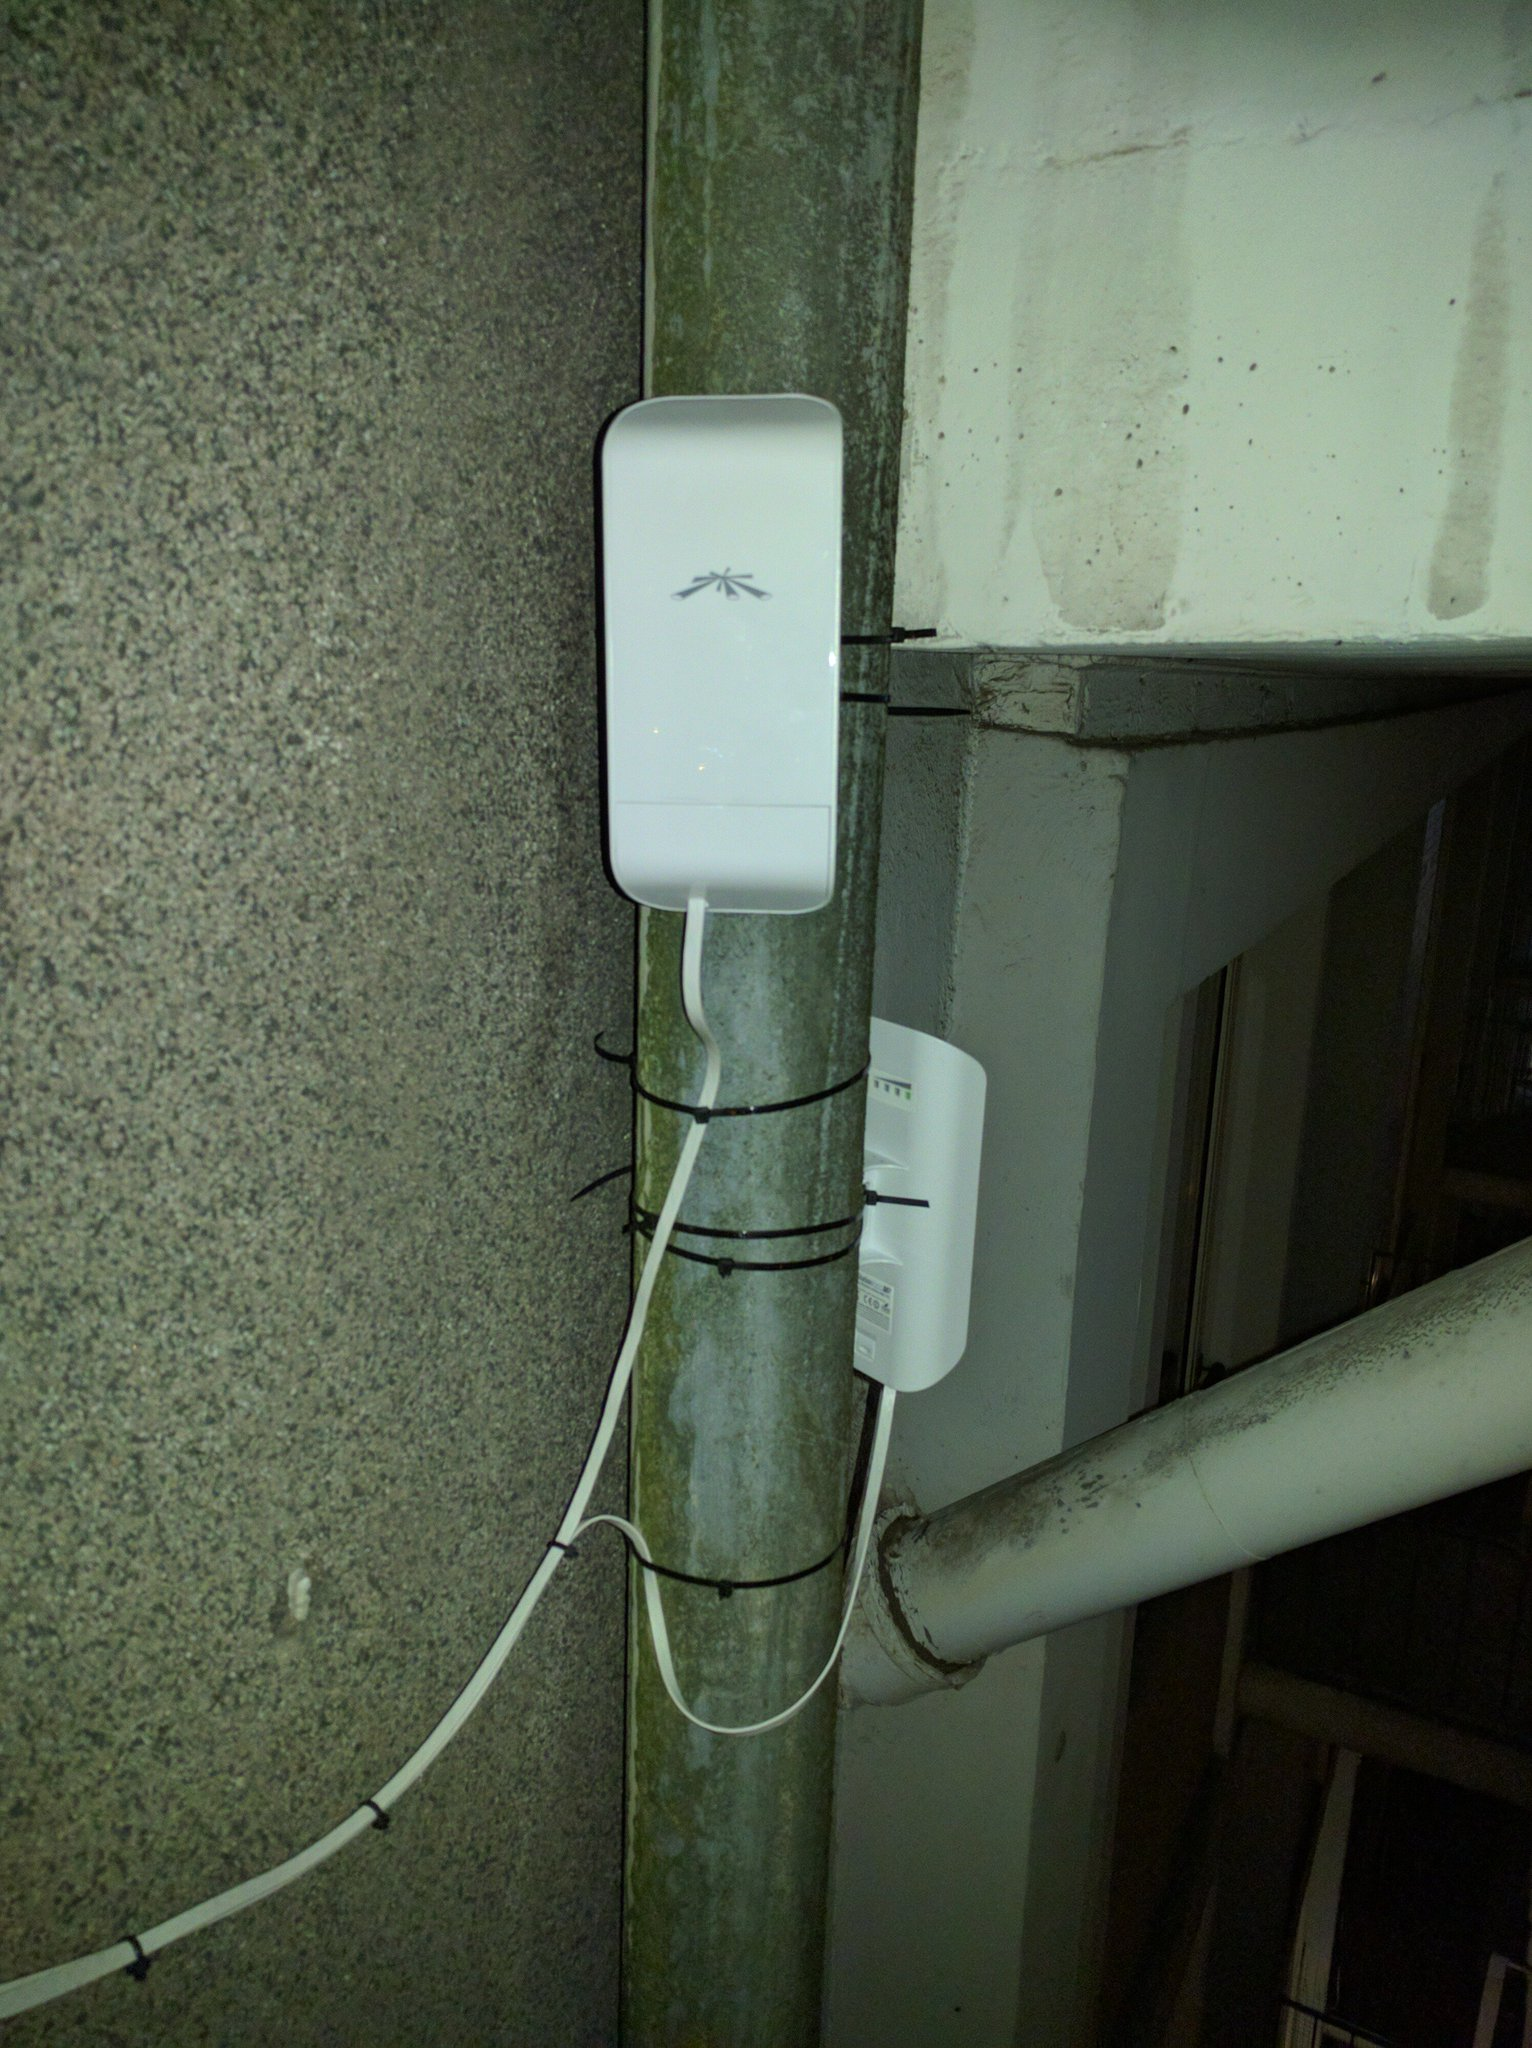
\includegraphics[width=5cm]{images/irl/wilhelminenstr2}
    \end{center}
  \end{frame}


  %-----------------
  \begin{frame}{Ohne Freifunk}
    \begin{center}
      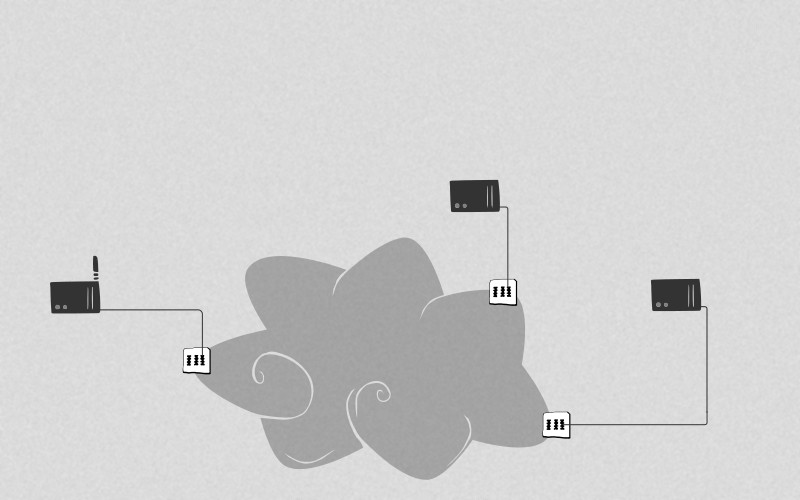
\includegraphics[height=5cm]{images/network_1}\\
      \vspace{1em}
      Geschlossene WLAN-Netze, welche nicht miteinander kommunizieren
      \vspace{1em}
    \end{center}
  \end{frame}

  %-----------------
  \begin{frame}{Mit Freifunk}
    \begin{center}
      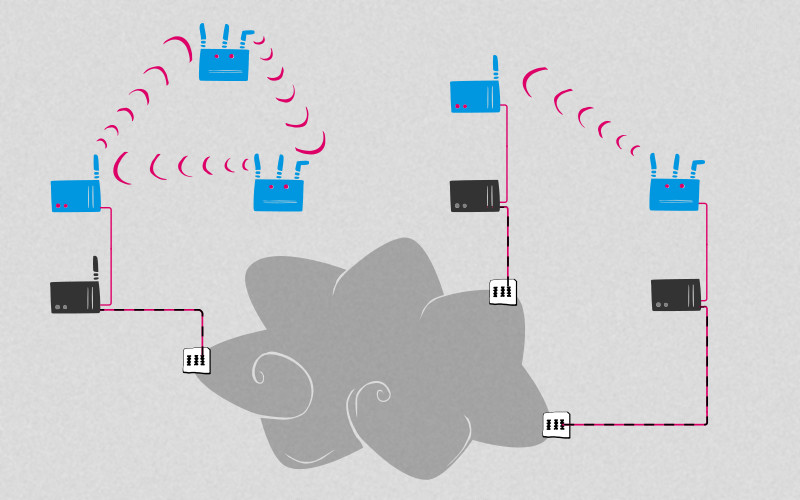
\includegraphics[height=5cm]{images/network_4}\\
      \vspace{1em}
      Freifunk-Knoten spannen ein freies Netz auf
      \vspace{1em}
    \end{center}
  \end{frame}


  %-----------------
  \begin{frame}{Richtfunknetz}
    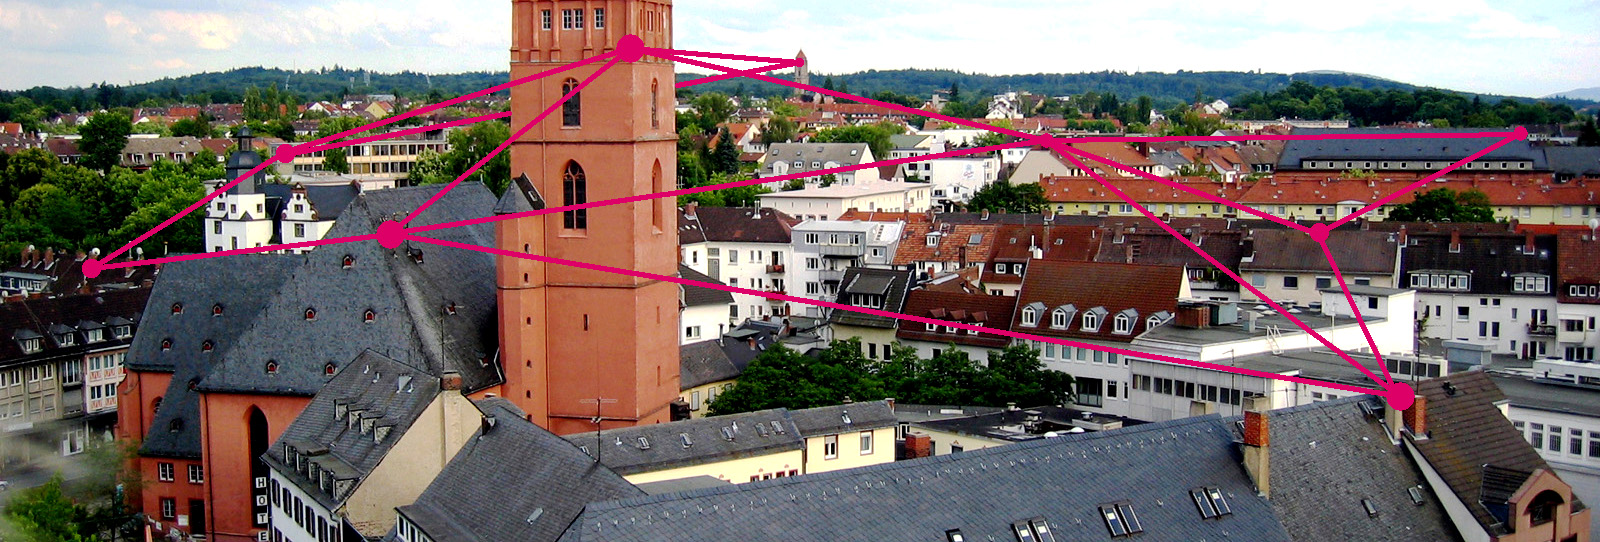
\includegraphics[width=\textwidth]{images/banner-stadtkirche-darmstadt}
    \begin{columns}
      \begin{column}{0.65\textwidth}
        \begin{itemize}
          \item Eigene Infrastruktur
          \begin{itemize}
            \item Redundanz und Lastverteilung
            \item Unabhängig vom Internet
          \end{itemize}
        \end{itemize}
      \end{column}
      \begin{column}{0.25\textwidth}
        \begin{center}
          \vspace{-1.5cm}
          \hspace{-0.75cm}
          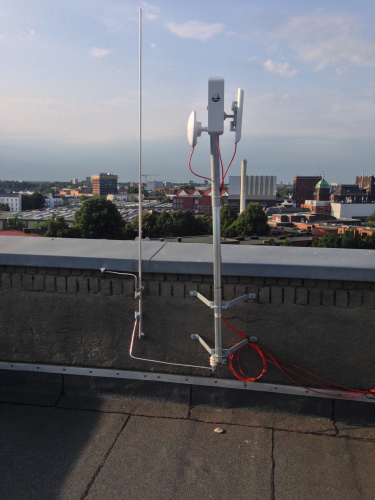
\includegraphics[width=\textwidth]{images/hamburg-richtfunkmast}
        \end{center}
      \end{column}
    \end{columns}
  \end{frame}


  %-----------------
  \begin{frame}{Ziele von Freifunk}
    \begin{itemize}
      \item \textbf{Beteiligung der Bevölkerung} an Aufbau und Entwicklung \textbf{dezentraler Netze}
      \item Verständnis von Kommunikationsnetzen fördern $\xRightarrow{}$ \textbf{Bildungsauftrag}
      \item Beteilung an gesellschaftlichen Initiativen, um die \textbf{Verbreitung freier Netze} zu unterstützen
    \end{itemize}
  \end{frame}


  %-----------------
  \begin{frame}{Verbreitung}
    \begin{columns}
      \begin{column}{0.6\textwidth}
        \begin{itemize}
          \item Deutschlandweit über  \href{http://freifunk.net/wie-mache-ich-mit/community-finden/}{\textbf{350} lokale Gruppen}
          \item mehr als \textbf{43.000} offene Zugangspunkte
        \end{itemize}
      \end{column}
      \begin{column}{0.4\textwidth}
        \begin{center}
          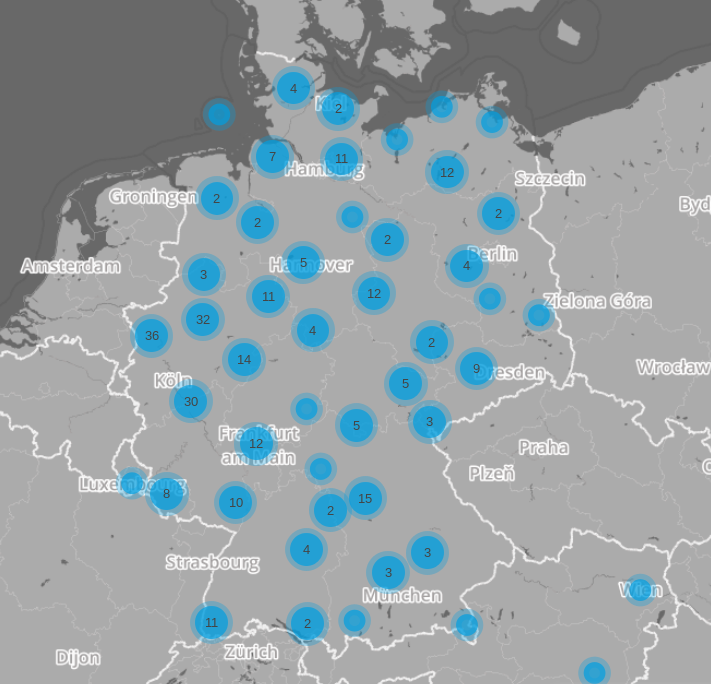
\includegraphics[width=\textwidth]{images/2016-06-01_map-de}
        \end{center}
      \end{column}
    \end{columns}
  \end{frame}


  %-----------------
   \begin{frame}{Freifunk Darmstadt: In Zahlen}
    \begin{itemize}
	  \item ungefähr 1600 gleichzeitige Nutzer täglich
	  \item \emph{über} 600 Freifunk-Knoten in Darmstadt und Umland
	  \item über 155 TB an Internetverkehr \emph{jeden Monat}
    \end{itemize}
    \begin{center}
      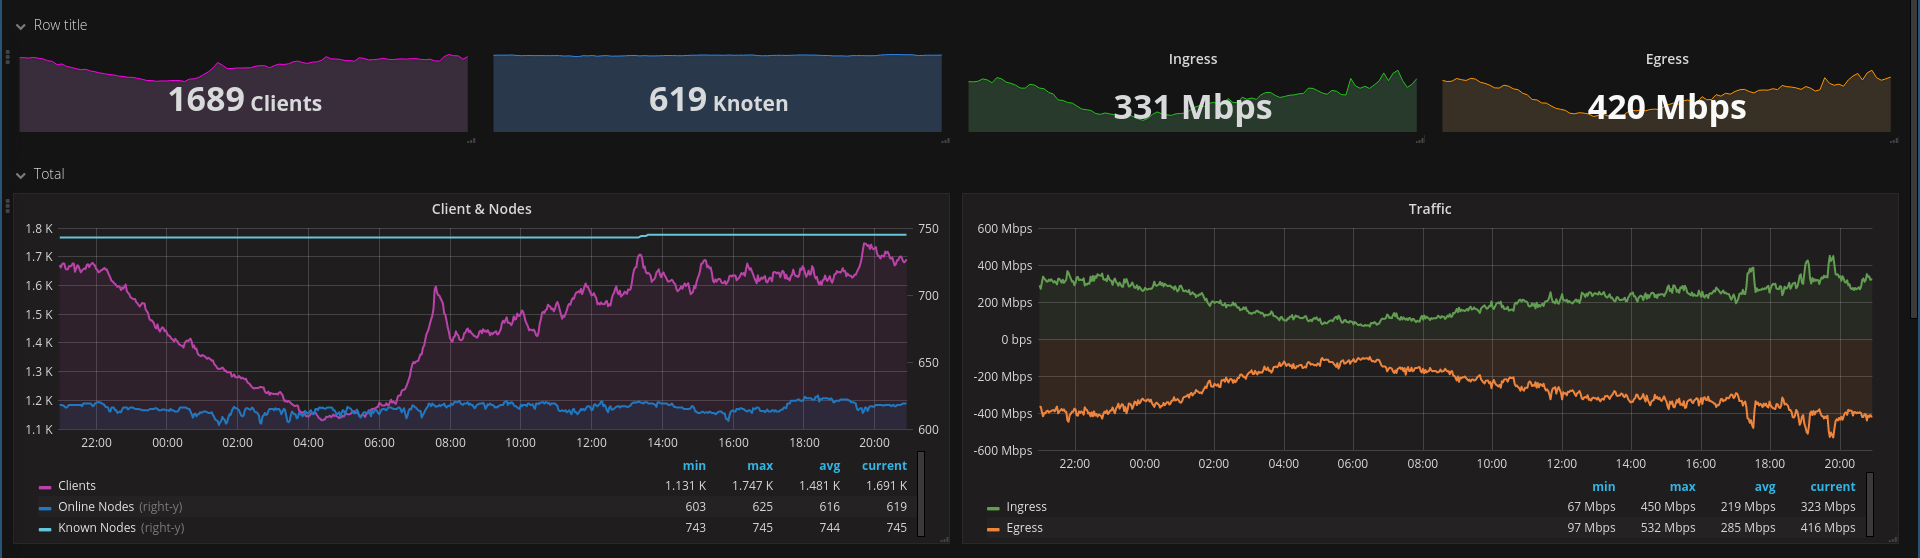
\includegraphics[height=3cm]{images/stats/grafana/2017_05_02}
    \end{center}
  \end{frame}


  %-----------------
  \begin{frame}{Stadt Darmstadt}
    \begin{itemize}
      \item September 2015: \textbf{Kooperation} mit OB Partsch, Stadt Darmstadt vereinbart
      \item Versorgung \textbf{aller angefragten Unterkünfte} mit WLAN
      \item Großartige Zusammenarbeit mit \textbf{ASB, DRK, Feuerwehr, Diakonie} und der Stadt
    \end{itemize}
  \end{frame}

  %-----------------
  \begin{frame}{Stadt Babenhausen}
    \begin{itemize}
      \item Versorgung einer Erstaufnahmeeinrichtung mit ca. \textbf{1.500 Personen} in ehem. US-Kaserne
      \item Versorgung der \textbf{Innenstadt} entlang der Hauptachse über 1,8 km
      \item \textbf{Beratung} des Bürgermeisters und tatkräftige Hilfe beim \textbf{Aufbau einer Community}
    \end{itemize}
  \end{frame}


  %-----------------
  \begin{frame}{Störerhaftung}
    \begin{columns}[T]
      \begin{column}{0.6\textwidth}
        \begin{itemize}
          \item Keine Haftung für \textbf{Knotenbetreiber}
          \item Internetverkehr geht über unsere Gateways. \textbf{Haftungsbefreiung} nach TMG \S8.
          \item Wir nehmen die gesetzlichen Vorschriften wörtlich: \textbf{Wir sammeln keine Daten}.
        \end{itemize}
      \end{column}
      \begin{column}{0.4\textwidth}
        \hspace{1em}
        
\includegraphics[width=\textwidth]{images/recht}
      \end{column}
    \end{columns}
  \end{frame}


  %-----------------
  \begin{frame}{Kosten}
    \begin{itemize}
      \item Ziel von Freifunk: \textbf{Kostenlose Teilnahme}
      \item Hardware je nach Nutzungsart \textbf{ab 25,- €}
      \item Infrastruktur für den Betrieb des Netzes kostet Geld!
      \begin{itemize}
        \item Betrieb der Internetanbindung, Strom, etc. nur durch \textbf{Sponsoren} möglich
      \end{itemize}
    \end{itemize}
  \end{frame}


  %-----------------
  \begin{frame}{Freifunk lebt vom Mitmachen}
    \begin{itemize}
      \item Freifunk ist \textbf{kein Dienstleister}
      \item Aufbau einer \textbf{lokalen Community} (falls nicht vorhanden) wünschenswert
      \item Andere Freifunk-Gruppen helfen gerne dabei und \textbf{geben Wissen weiter}
    \end{itemize}
    \begin{center}
      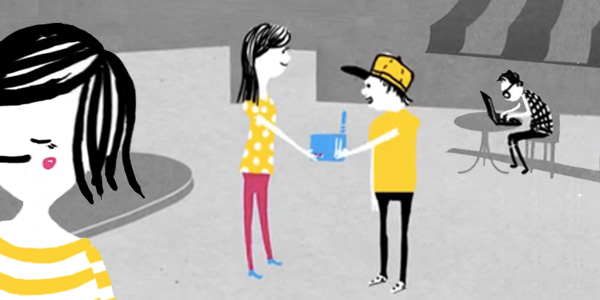
\includegraphics[height=0.28\textheight]{images/router}
      \hspace{0.5em}
      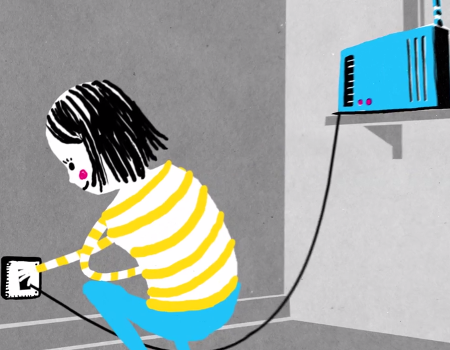
\includegraphics[height=0.28\textheight]{images/setup}
    \end{center}
  \end{frame}


  %-----------------

  \begin{frame}{Vielen Dank!}
    \begin{textblock*}{0cm}(\textwidth-2cm,-2cm)
      \begin{figure}[h]
        \def\svgwidth{2.5cm}
        \input{logo.pdf_tex}
      \end{figure}
    \end{textblock*}
      \begin{itemize}
        \item Webseite: \href{http://darmstadt.freifunk.net/}{darmstadt.freifunk.net}
        \item E-Mail: \href{info@darmstadt.freifunk.net}{info@darmstadt.freifunk.net}
        \item Treffen: Jeden Montag um 19:00 Uhr
        \begin{itemize}
          \item im Hackspace des Chaos Darmstadt e.V.
          \item Wilhelminenstr. 17, 64283 Darmstadt
        \end{itemize}
      \end{itemize}
      \vspace{1em}
  \end{frame}
\end{document}
